\section{Current Results and Validation}
\label{sec:results}

We report topology and downstream validity separately because a visually clean mesh can be unusable if it contains even one phase-shortcut fusion.

\begin{figure*}[t]
  \centering
  \begin{subfigure}[b]{0.48\linewidth}
    \centering
    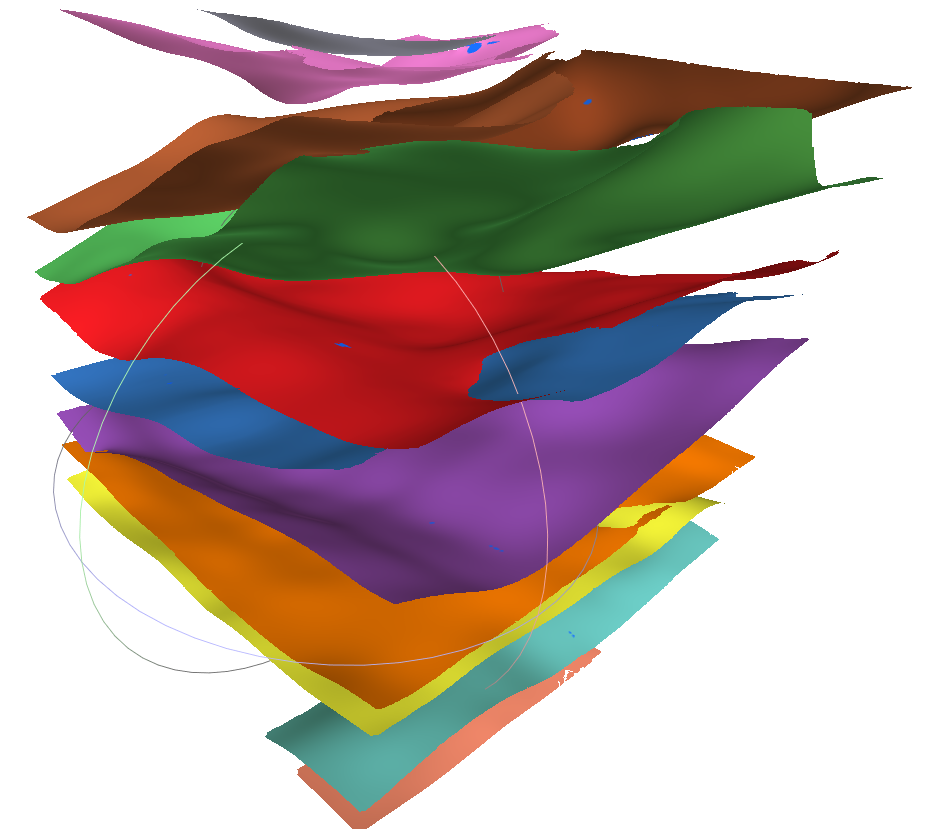
\includegraphics[width=\linewidth]{figures/kaggle_cube_118632705.png}
    \caption{Source cube 118632705 (11 sheets)}
    \label{fig:kaggle_a}
  \end{subfigure}
  \hfill
  \begin{subfigure}[b]{0.48\linewidth}
    \centering
    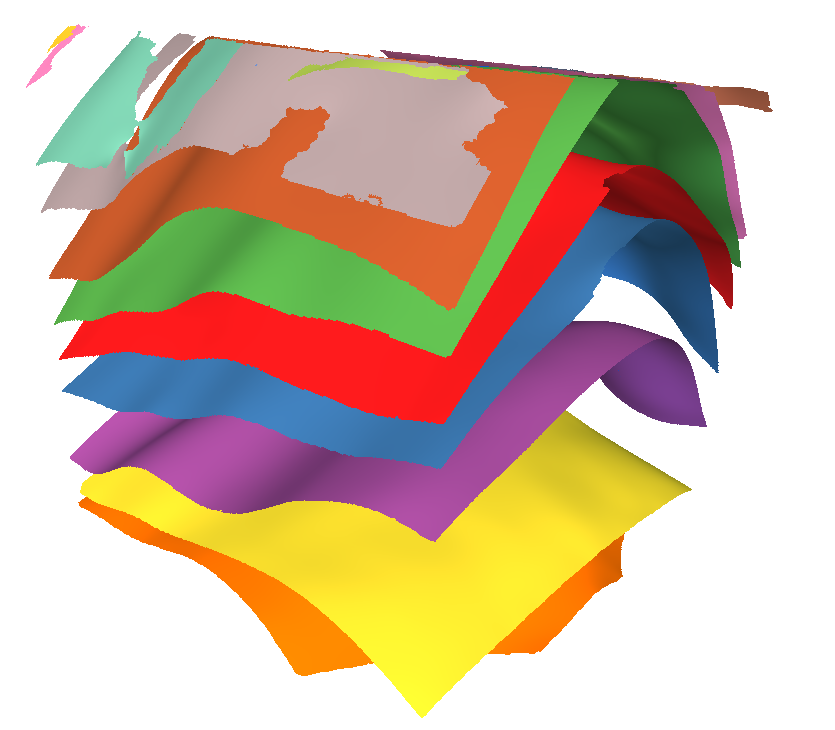
\includegraphics[width=\linewidth]{figures/kaggle_cube_3394433588.png}
    \caption{Source cube 3394433588 (15 sheets)}
    \label{fig:kaggle_b}
  \end{subfigure}
  \caption{Two dense Vesuvius Challenge training cubes after single-sided reconstruction and overlap separation. The roughly two-million-point inputs are divided into 11 and 15 component-coloured sheets before the current CVT/RVD level-of-detail stage.}
  \Description{Two coloured triangle-mesh stacks showing many separated, approximately parallel papyrus sheets in dense voxel cubes.}
  \label{fig:kaggle_cubes}
\end{figure*}

\begin{figure*}[t]
  \centering
  \begin{subfigure}[b]{0.360\linewidth}
    \centering
    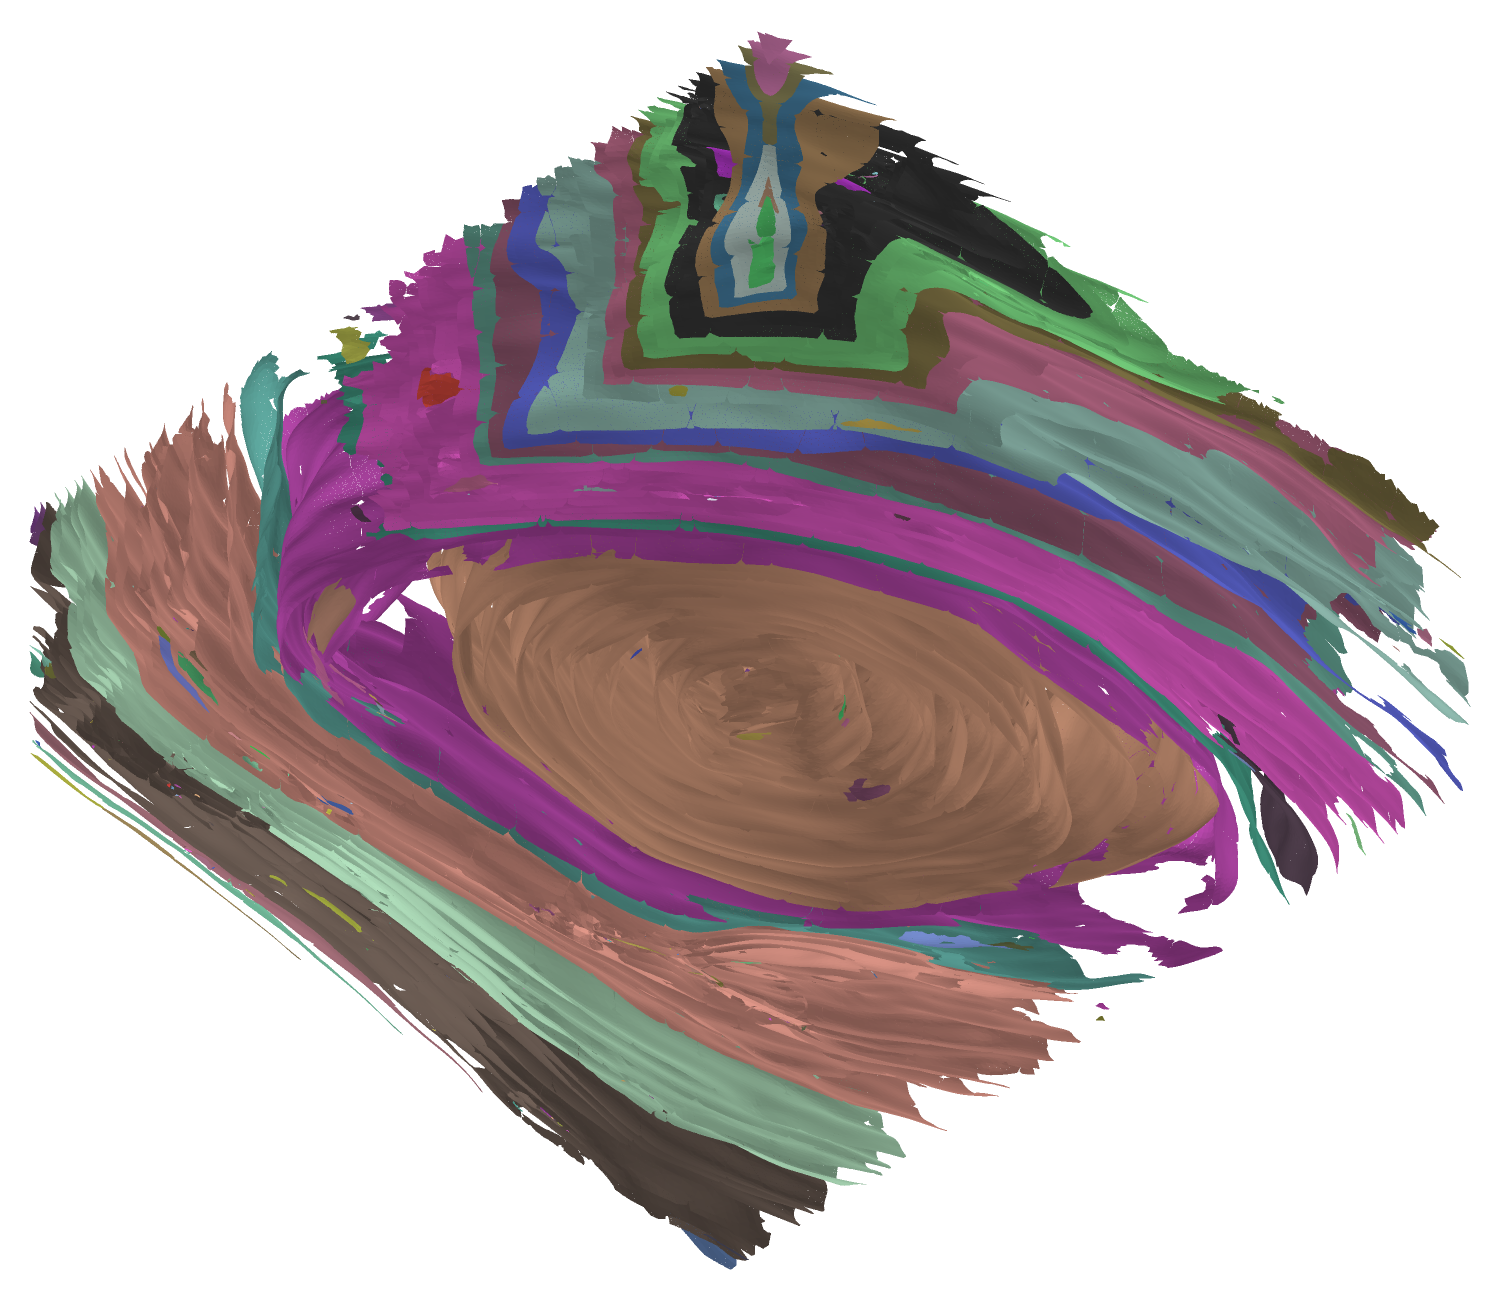
\includegraphics[width=\linewidth]{figures/mesh_10x10x10.png}
    \caption{PHerc0139, $10\times10\times10$ cubes: geometry}
    \label{fig:scale_10x_mesh}
  \end{subfigure}
  \hfill
  \begin{subfigure}[b]{0.620\linewidth}
    \centering
    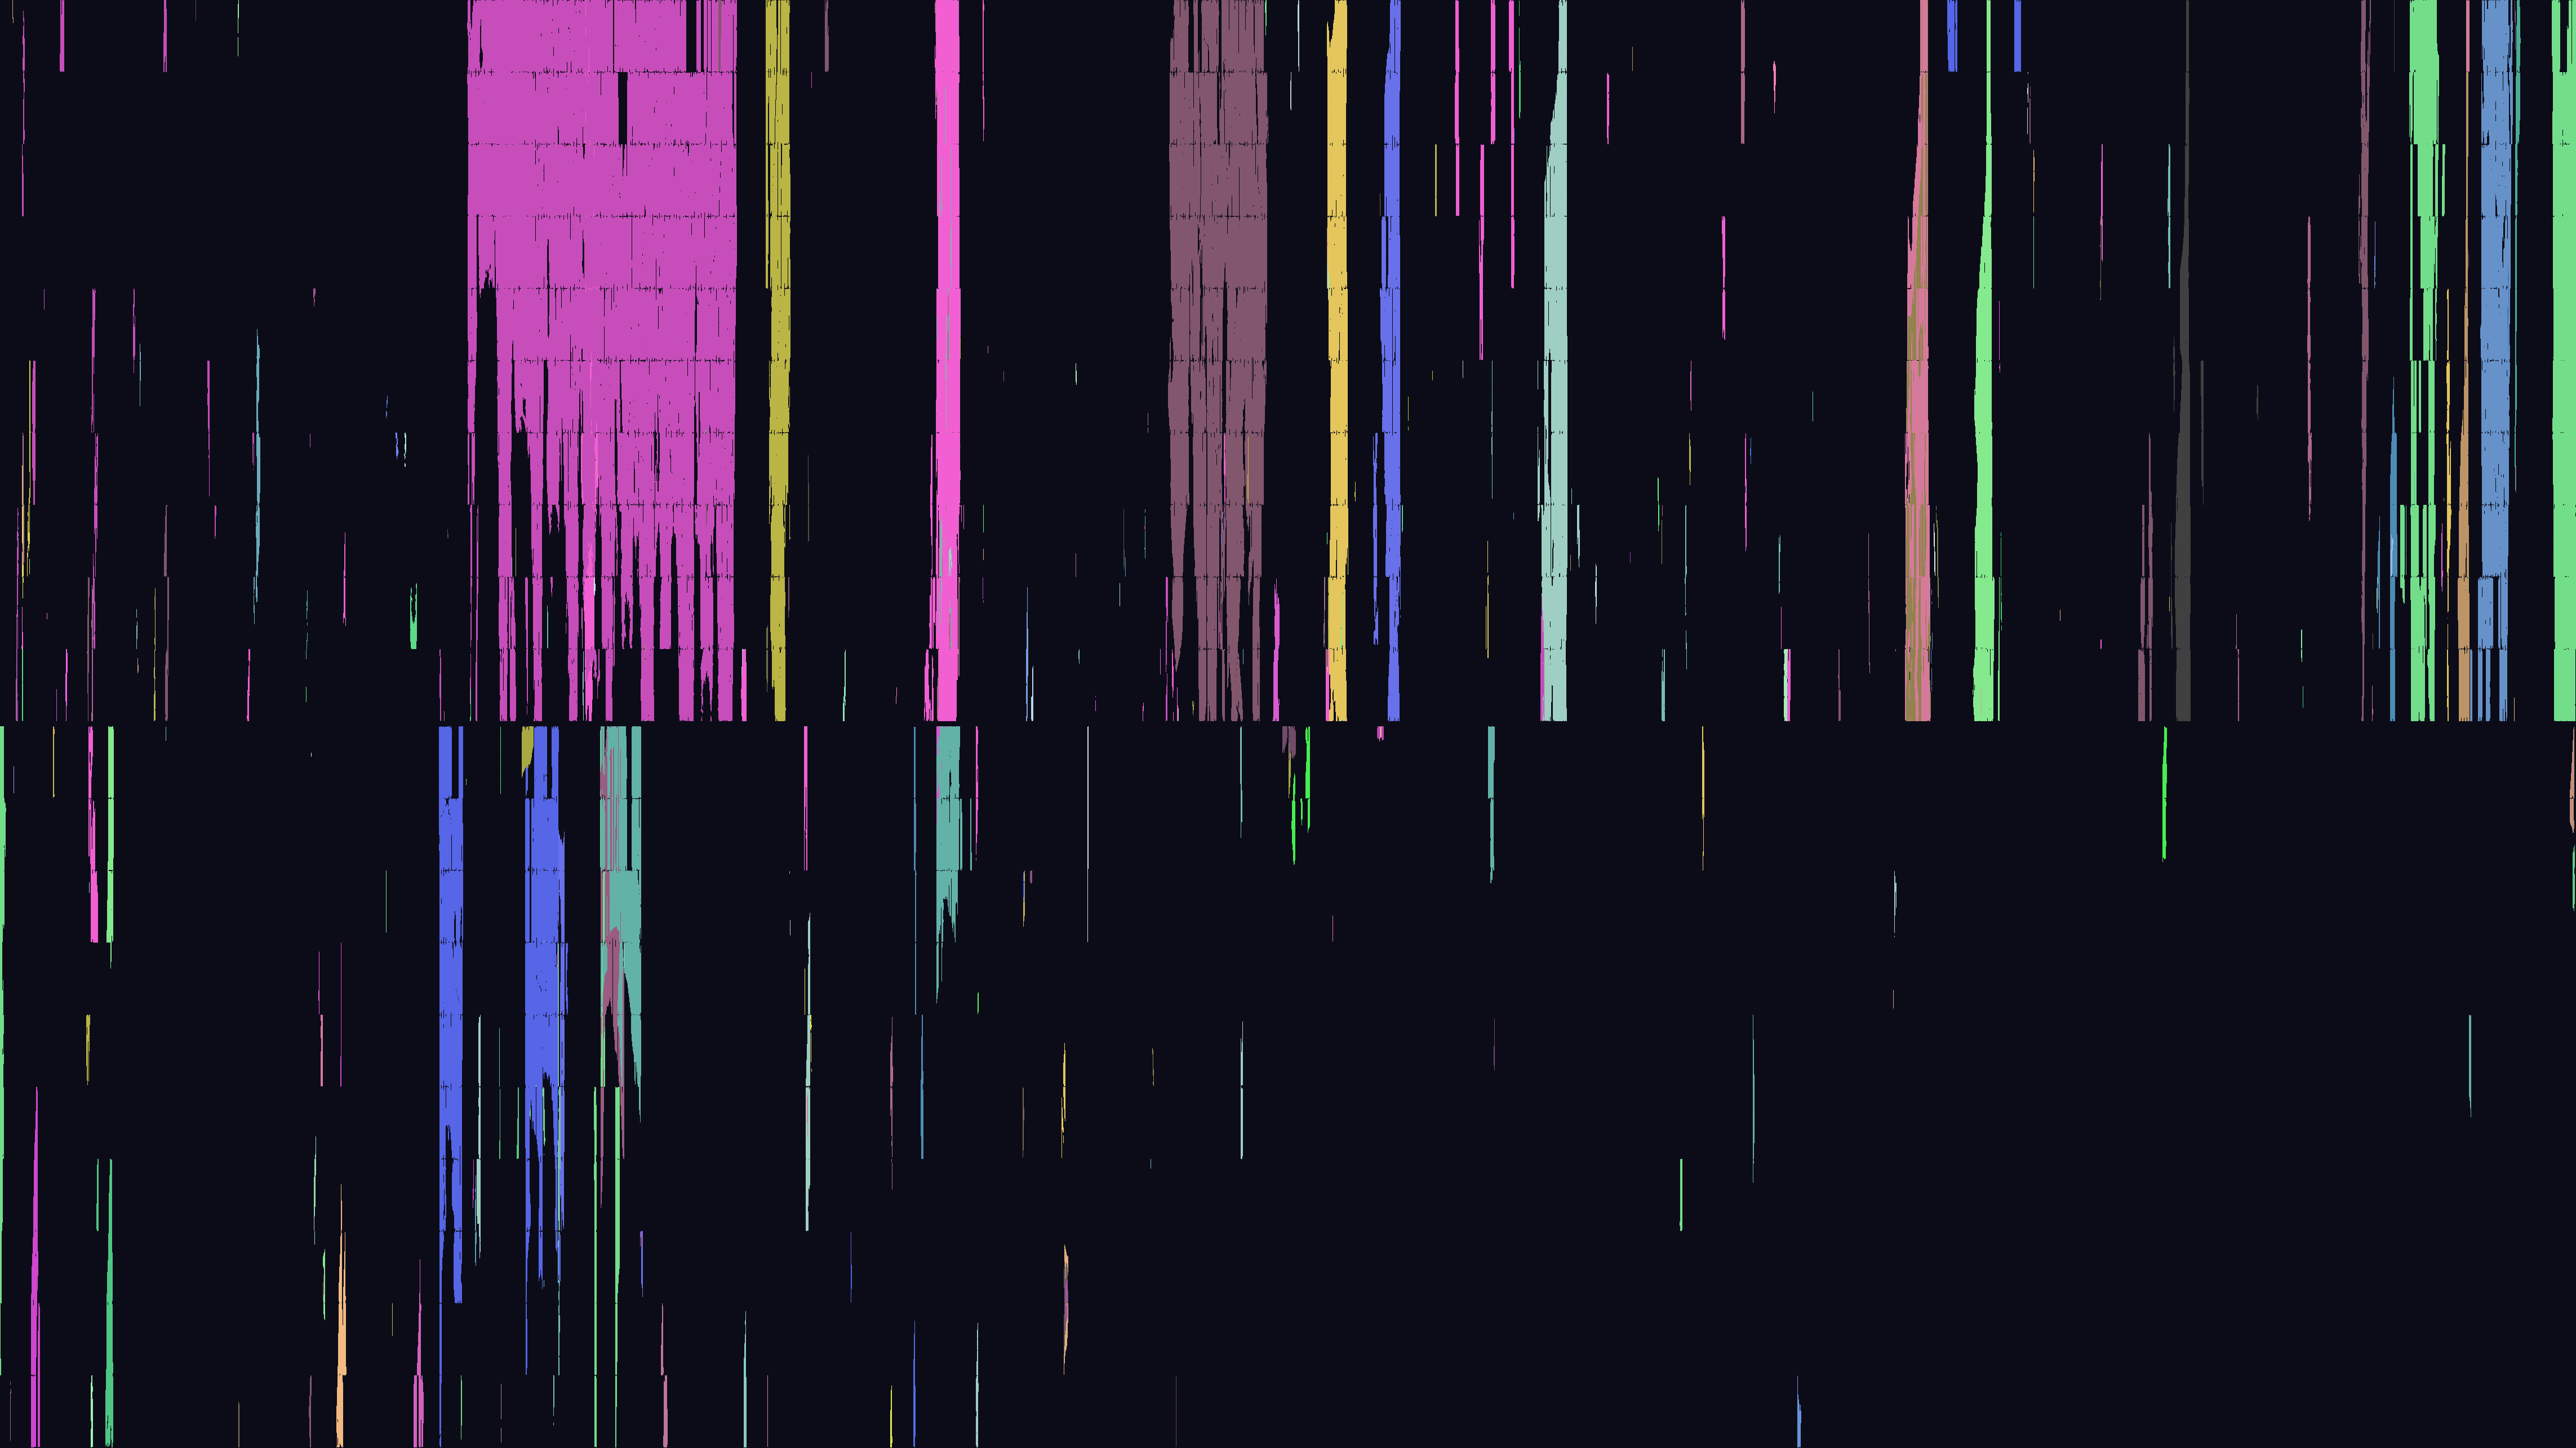
\includegraphics[width=\linewidth]{figures/atlas_10x10x10.png}
    \caption{PHerc0139, $10\times10\times10$ cubes: the registered atlas, cut into two rows}
    \label{fig:scale_10x}
  \end{subfigure}

  \medskip
  \begin{subfigure}[b]{0.735\linewidth}
    \centering
    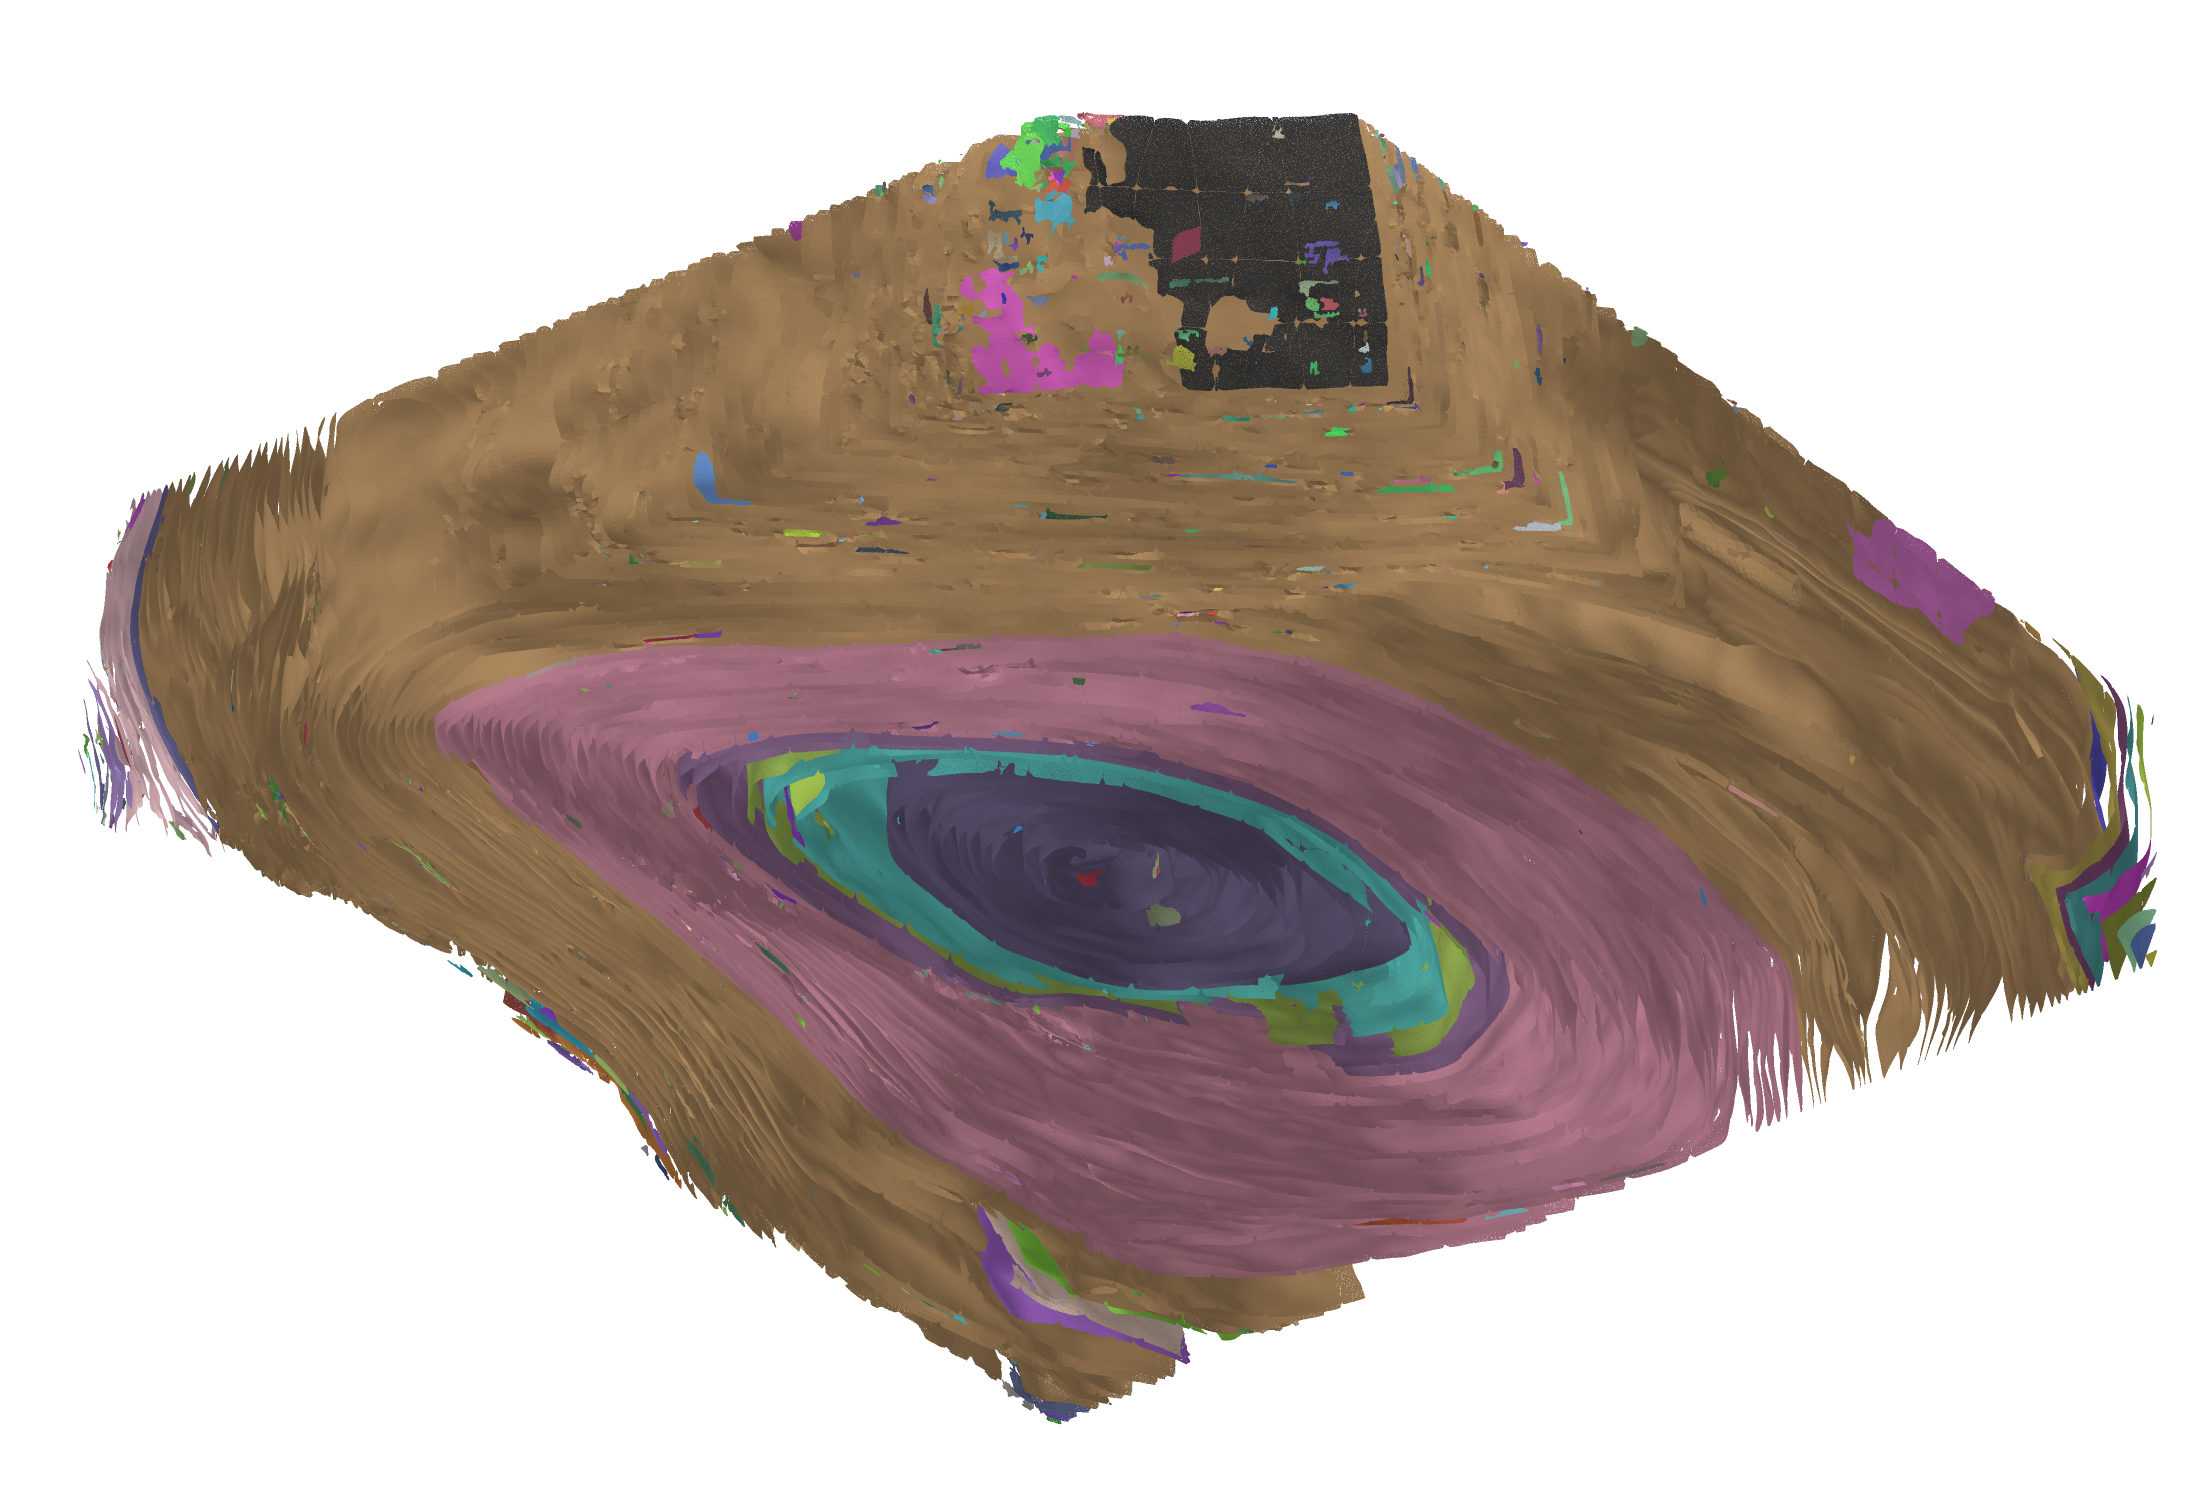
\includegraphics[width=\linewidth]{figures/mesh_4x21x21.png}
    \caption{PHerc0139, $4\times21\times21$ cubes: the band geometry (1,702 cubes)}
    \label{fig:scale_21x_mesh}
  \end{subfigure}
  \hfill
  \begin{subfigure}[b]{0.245\linewidth}
    \centering
    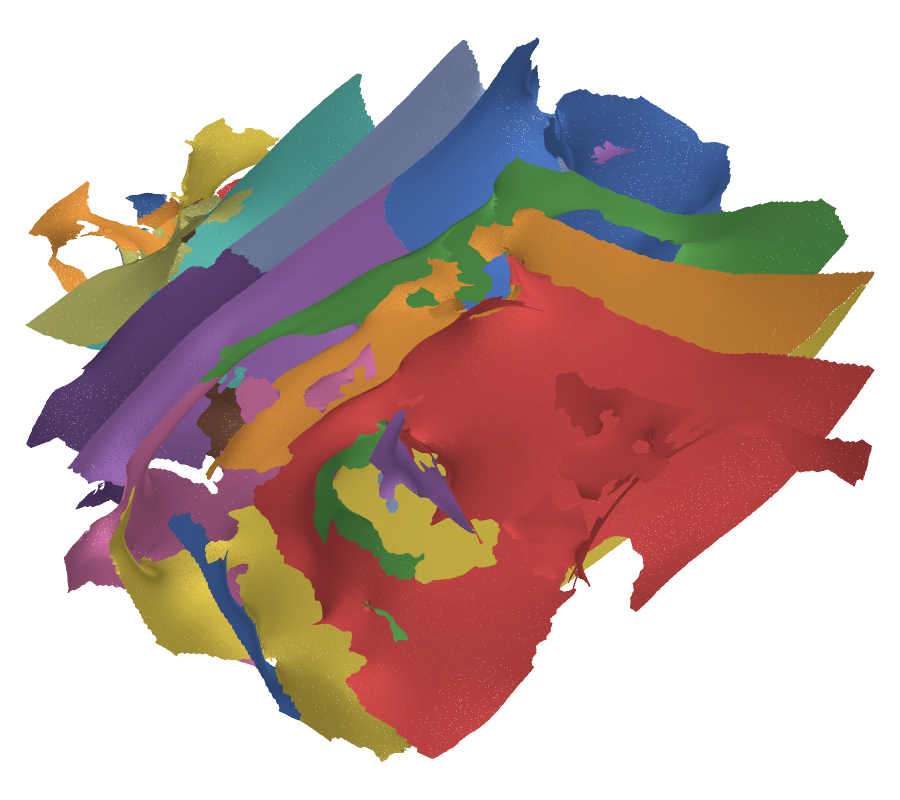
\includegraphics[width=\linewidth]{figures/pherc1203_cube.png}
    \caption{PHerc1203, one reconstructed cube}
    \label{fig:scale_1203}
  \end{subfigure}
  \caption{The same implementation beyond the $4\times5\times5$ fixture. (a) The thousand-cube PHerc0139 block in world space, cut at mid-height along the scroll axis to expose the recovered wraps spiralling around the umbilicus; colour identifies the welded atlas group, as in (b). (b) The same block carried through registration and the winding lift: the large welded groups survive as contiguous single-colour regions separated along $u$, which is the property the lift exists to produce, while the sparser second row is the volume's tail. (c) The full $4\times21\times21$ band --- 1,702 reconstructed cubes in world space, coloured by welded group, the geometry behind the stripwise atlas experiments. (d) A PHerc0139-trained configuration applied unchanged to a PHerc1203 cube, separated into component-coloured single-sided sheets. These runs demonstrate that the path scales and transfers; the winding and collision gates of Section~\ref{sec:repair} have not yet been run at these sizes.}
  \Description{Four panels: a cutaway render of a large spiral scroll block with wraps in distinct group colours, a wide two-row raster of a large unrolled atlas with contiguous coloured regions, a long slab-shaped render of many concentric papyrus wraps coloured by group, and a component-coloured render of separated sheets in a single reconstructed cube from a different scroll.}
  \label{fig:scale}
\end{figure*}

\paragraph{Per-cube extraction.}
Figure~\ref{fig:kaggle_cubes} shows two dense training cubes (source IDs 118632705 and 3394433588) with 2.07M and 1.92M raw points. Guarded BPA and the overlap separator recover 11 and 15 distinct single-sided sheets. Bridge separation and hole repair are shown in Fig.~\ref{fig:bridgesplit}. Across a difficult {\em PHerc1447} probe, however, adaptive BPA radii 1.20, 1.10, and 1.00 all retained nine broad fusions with maximum local span 18.70 turns while the boundary count increased. The quality gate therefore rejects radius reduction as a solution and requires those regions to be cut or quarantined.

\paragraph{Current 100-cube weld and CVT/RVD}
The latest complete central $4\times5\times5$ rebuild of {\em PHerc0139} processed all 100 cubes into a 264,268-face welded mesh (Fig.~\ref{fig:overview_mesh}), compared with 3.02M faces in the earlier collapse-only build. It has zero non-manifold edges and five same-direction edges. In the seam-band A/B, pinned CVT/RVD raised mean minimum triangle angle from $38.70^\circ$ to $43.38^\circ$, reduced triangles below $30^\circ$ from 24.88\% to 11.73\%, and changed 366,185 faces to 262,659 while preserving the audited boundary, component, Euler, and manifold counts exactly.

Those local topology counts do not certify scroll phase. The strict winding audit found 6,082 abrupt full-turn fusion edges; only 9.37\% lie near cube seams, which identifies prediction and per-cube reconstruction as the dominant source rather than welding. The experimental phase sever removed 9,650 faces (3.7\%), changed 28 connected components to 122, and reduced the abrupt-edge count to zero. Some resulting components still fail the broad local-span audit, so this output is exported only as an unverified hint. This negative result is important: manifoldness, orientation, and good triangles are necessary but not sufficient for a readable scroll.

\paragraph{Verified local flattening.}
On a clean 6,302-face {\em PHerc1447} component, the ScrollFiesta ribbon, quilting, and snap stages produced 21,218 valid cells, 20,873 valid quads, and no contested cells. The final output of Villa's maintained \texttt{flatboi} flattener contained 20,697 valid cells and 20,349 valid quads; the solve converged in five iterations, 87.1\% of the output grid rasterized, and the official loader, surface-index overlap connector, and full Spiral load-only path passed. By contrast, our optional relaxation left five flipped faces and changed mean stretch from 1.0298 to 1.0617, supporting the decision to delegate verified final flattening to Villa.

\paragraph{Geometric strip correction.}
The new audit found that 8,320 of 9,744 original plane-slice strokes traversed at least half a wrap internally, with a maximum span of 8.75 turns. Cutting 8,741 chains at 44,911 geometric wrap crossings produced 33,858 fragments; only 198 still span half a turn, and the maximum residual span is 0.68. The metric solve then changed developed advance per radial turn from 10.3\% to 103.1\% of a circumference. For comparison, posing the same monotone-constrained system as one large active-set QP hits a 235-second iteration cap without converging on the fragmented post-cut system, where the reduced LS--PAVA solve completes 11-round solves in 4.8--8.8 seconds. Direct-support transfer removed 2,304 of 172,116 candidate faces (1.34\%), including every one of the 696 zero-area UV faces that had survived neighbour filling. The corrected 169,812-face field has no degenerate UV triangle, no aspect ratio above 50, and no UV edge stretched more than $4\times$ its corresponding 3D edge. Rigid chart application preserves these local differences exactly.

\paragraph{Tabu winding repair.}
The locally metric field was still globally collapsed: 84.6\% of its within-group overlap pairs lay at least 0.75 pitch apart in radius, indicating different wraps at the same $u$. Table~\ref{tab:tabu} summarizes the discrete repair. The first per-chart search removed 95.4\% of exact overlaps but tore too many weld relations. Measuring the real field's wind ladder, adding same-wind lateral and happy-family terms, alternating with metric re-registration, and finally deriving graded bins from the weld chain reduced the exact count to 472 cross-group plus 1,402 within-group pairs, or 1,874 total (99.5\% below the registered field). A problematic 22-chart group's wrong-wind internal count fell from roughly 38,000 to 2, a second fell to zero, and the 324-chart group's count fell from 61,016 to 757. No happy-family bond tore; 41 usable weld relations remain torn and are the focus of the current stabilization work.

\begin{table}[t]
  \caption{Exact UV triangle-overlap progression on the $4\times5\times5$ atlas. ``Torn'' counts usable weld relations whose final integer-depth difference misses its target.}
  \label{tab:tabu}
  \centering
  \small
  \begin{tabular}{@{}lrrr@{}}
    \toprule
    Stage & Cross & Within group & Torn \\
    \midrule
    Registered field & 241,078 & 132,458 & 0 \\
    Per-chart tabu & 172 & 17,109 & 167 \\
    Alternating + graded & 535 & 3,447 & 38 \\
    Weld-chain bins & 472 & 1,402 & 41 \\
    \bottomrule
  \end{tabular}
\end{table}

The independent confirmation does not rely on the pair count alone. A four-round atlas bake produced a 47,514-by-511 CT strip with 30.4\% fill and 0.15\% multiple coverage; papyrus fabric remains continuous across chart seams. Per-winding OBJ layers show whether one colour moves coherently, while the $u$-radius plot separates formerly stacked winds. The exact-SAT stabilization work additionally records physical weld mismatch, because an integer target can look satisfied while the final seam is displaced by tens or hundreds of voxels; closing these stricter acceptance checks and establishing a verified global order of the separated group bands are the remaining steps.

An earlier $4\times21\times21$ band (Fig.~\ref{fig:scale_21x_mesh}) was parameterized as four axial strips using one winding calibration. Exact \texttt{tifxyz} welding retained 51,469,897 valid pixels across 166 wraps, with continuous fibres at strip boundaries, and arc registration reduced controlled seam texture mismatch by four to six times. That long band has not yet been rerun through the new global tabu stage. The $4\times5\times5$ VC3D demonstration carried a 544,178-cell unverified hint into Spiral feedback; a second correction reduced the active hint loss from 81.0648 to 13.0018 (83.96\%) and improved symmetric RMS by 10.31\%. These numbers measure the feedback channels; the underlying core surface is gated separately.

\paragraph{Snap and RAW-guided repair.}
Figure~\ref{fig:snap} demonstrates the present behaviour: supported dark islands move onto a coherent papyrus signal while anchorless cracks remain. The first-stage graph cut, occupancy barrier, joint quilting target, and screened solve are implemented in the pipeline; the oriented recto-transition pass is also implemented and undergoing real-volume comparison. The remaining failures concentrate in folded, delaminated core geometry, where candidate direction and ownership are ambiguous; the correction stays conservative there, and every vertex displacement is individually revertible.

\paragraph{Performance and backend parity.}
An OpenMP/MLS engine rewrite reduced one recorded $4\times5\times5$ mesh stage from 1,996\,s to 88.7\,s with byte-identical output, and removal of two hidden quadratic searches reduced the corresponding weld kernel from 351\,s to 79\,s, also byte-identically. The latest complete build meshed its 100 cubes in 129.2\,s and completed the full weld in approximately 9.3 minutes; pinned band CVT/RVD is now the dominant cost. On a captured 399,741-point {\em PHerc1447} cloud, five CubeCL CUDA MLS passes took a median 234.741\,ms and differed from the C reference by at most 0.000594 voxels. A complete-cube comparison took 73.654\,s versus 488.211\,s for the C path, approximately $6.6\times$ faster, while retaining the same downstream audits.

